\documentclass[10pt,a4paper]{article}
\usepackage[margin=2cm]{geometry}
\usepackage[T1]{fontenc}
\usepackage{lmodern}
\usepackage{amsmath,amssymb}
\usepackage{booktabs,tabularx}
\usepackage{enumitem}
\usepackage[dvipsnames]{xcolor}
\usepackage{listings}
\usepackage{tikz}
\usetikzlibrary{arrows.meta,positioning}
\usepackage[most]{tcolorbox}
\usepackage[colorlinks=true,linkcolor=blue!60!black,urlcolor=blue!60!black]{hyperref}

\setlist{nosep,leftmargin=1.2em}
\setlength{\parindent}{0pt}
\setlength{\parskip}{4pt}
\newcommand{\code}[1]{\texttt{\detokenize{#1}}}
\newtcolorbox{keybox}[1]{colback=blue!3,colframe=blue!45!black,fonttitle=\bfseries,title=#1,boxrule=0.6pt,arc=1mm,left=4pt,right=4pt,top=2pt,bottom=2pt}
\newtcolorbox{notebox}{colback=orange!5,colframe=orange!70!black,boxrule=0.6pt,arc=1mm,left=4pt,right=4pt,top=2pt,bottom=2pt}

\lstset{language=Matlab,basicstyle=\ttfamily\small,keywordstyle=\color{blue!70!black},
  commentstyle=\color{green!45!black},stringstyle=\color{purple!80!black},
  frame=single,rulecolor=\color{black!25},backgroundcolor=\color{black!2},
  columns=fullflexible,keepspaces=true,upquote=true,showstringspaces=false,
  xleftmargin=2pt,xrightmargin=2pt,aboveskip=4pt,belowskip=4pt}
\tikzset{blk/.style={draw,thick,minimum height=8mm,minimum width=12mm,align=center,font=\small},
  sum/.style={draw,thick,circle,minimum size=5mm,inner sep=0pt},
  sig/.style={-{Latex[length=2mm]},thick}, lbl/.style={font=\scriptsize}}

\title{\textbf{The feedforward fit, explained}\\[2pt]\large \code{scripts/control/ff_correct.m}: theory and code, line by line}
\date{}
\begin{document}
\maketitle
\vspace{-8mm}

\begin{keybox}{In one paragraph}
The feedforward gives the motor the voltage it needs to follow the path; the feedback corrects what is missing, and it can
do so only through an error. If the motor model behind the feedforward is wrong, an error stays. \code{ff_correct.m} takes
a run, measures how much voltage the motor \emph{really} needed to follow the path, fits the three parameters of the
feedforward ($k$, $\tau$, $V_c$) to that voltage, and writes them for the next run. The loop (poles, margins) is not touched.
\end{keybox}

%==========================================================================================
\section{Why there is a tracking error, and why the feedforward removes it}

\begin{center}
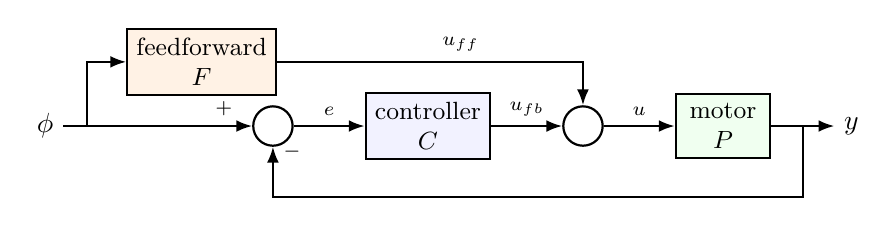
\begin{tikzpicture}[node distance=6mm and 9mm]
  \node (r) {$\phi$};
  \node[blk,above right=1mm and 8mm of r,fill=orange!10] (ff) {feedforward\\ $F$};
  \node[sum,right=24mm of r] (se) {};
  \node[blk,right=of se,fill=blue!5] (c) {controller\\ $C$};
  \node[sum,right=of c] (su) {};
  \node[blk,right=of su,fill=green!6] (p) {motor\\ $P$};
  \node[right=8mm of p] (y) {$y$};
  \draw[sig] (r) -- node[lbl,above,pos=0.85]{$+$} (se);
  \draw[sig] (r.east) ++(3mm,0) |- (ff.west);
  \draw[sig] (se) -- node[lbl,above]{$e$} (c);
  \draw[sig] (c) -- node[lbl,above]{$u_{fb}$} (su);
  \draw[sig] (ff.east) -| node[lbl,above,pos=0.3]{$u_{ff}$} (su.north);
  \draw[sig] (su) -- node[lbl,above]{$u$} (p);
  \draw[sig] (p) -- coordinate[pos=0.5](yy) (y);
  \draw[sig] (yy) |- ++(0,-9mm) -| node[lbl,right,pos=0.95]{$-$} (se.south);
\end{tikzpicture}
\end{center}

With a feedforward $F$ and a controller $C$ on the motor $P$, the tracking error is
\begin{equation}\label{eq:err}
  e=\phi-y=\underbrace{\frac{1}{1+PC}}_{S}\,\bigl(1-PF\bigr)\,\phi .
\end{equation}
\begin{itemize}
  \item If $F=P^{-1}$ (the feedforward is the exact inverse of the motor), then $1-PF=0$ and $e=0$ for \emph{any} path: the
        feedforward alone moves the motor, the feedback has nothing to do.
  \item If $F$ is built on a wrong model, $1-PF\neq0$: the feedback must supply the difference, and it does so only through
        $e$. The error is reduced by $S$ (small at low frequency, thanks to the integral action) but not removed.
  \item $F$ does not appear in $S$: changing the feedforward never changes stability, poles or margins.
\end{itemize}
So the goal is a feedforward as close as possible to $P^{-1}$, and the best place to learn $P^{-1}$ is the plant itself.

%==========================================================================================
\section{The model of the voltage}

\textbf{Motor.} Each joint is a DC motor with its load: $\tau\ddot\theta_m+\dot\theta_m=k\,u$ ($\theta_m$ in rad, motor sign).
The encoder counts the opposite way, so the joint angle used everywhere is $\phi=-\theta_m$ (converted to degrees for the
reference). The voltage that moves the joint along $\phi(t)$ is the inverse of the model:
\begin{equation}\label{eq:inv}
  u(t) = -\frac{1}{k}\dot\phi(t)-\frac{\tau}{k}\ddot\phi(t) \qquad(\dot\phi,\ddot\phi\ \text{in rad/s, rad/s}^2).
\end{equation}
The first term pushes against the viscous friction and back-EMF (it grows with speed), the second accelerates the inertia.

\textbf{Friction.} Coulomb friction is a constant torque opposing the motion, i.e.\ a constant voltage
$V_c\,\mathrm{sign}(\dot\theta_m)$. $\mathrm{sign}$ jumps at zero speed; $\tanh(\dot\phi/w_\varepsilon)$ is the same curve with
a smooth step of width $w_\varepsilon=0.02$ rad/s, so the voltage has no jump when a joint reverses.

\textbf{Offset.} A constant $c_4$ collects anything constant (an amplifier offset, a mean load torque); keeping it in the
fit prevents it from leaking into the other coefficients.

\textbf{Delay.} If the voltage reaches the motor $T_d$ seconds late, the feedforward should anticipate it: the voltage needed
at time $t$ is the one for $\phi(t+T_d)\approx\phi(t)+T_d\dot\phi(t)$. Putting this in \eqref{eq:inv}:
\begin{equation}
  -\frac{1}{k}\bigl(\dot\phi+T_d\ddot\phi\bigr)-\frac{\tau}{k}\ddot\phi
  =-\frac{1}{k}\dot\phi-\frac{\tau+T_d}{k}\ddot\phi .
\end{equation}
A small delay looks exactly like a larger time constant: the fit finds $\tau_{ff}\approx\tau+T_d$ and compensates it without
modelling the delay explicitly.

\textbf{All together}, the voltage is \emph{linear in four unknown coefficients}:
\begin{equation}\label{eq:model}
  u = c_1\dot\phi + c_2\ddot\phi + c_3\tanh\!\left(\frac{\dot\phi}{w_\varepsilon}\right) + c_4,
  \qquad
  k=-\frac{1}{c_1},\quad \tau=\frac{c_2}{c_1},\quad V_c=-c_3 .
\end{equation}
The last three relations come from matching \eqref{eq:model} with the feedforward of the Simulink models,
$u_{ff}=-\frac{1}{k_{ff}}\dot\phi-\frac{\tau_{ff}}{k_{ff}}\ddot\phi-V_{c,ff}\tanh(\dot\phi/w_\varepsilon)$.

%==========================================================================================
\section{Why the logged voltage is the right data}

The controller voltage is $u=u_{ff}+u_{fb}$. After the start, the joint follows the path closely ($y\approx\phi$, errors of a
fraction of a degree). The motor obeys its own dynamics: whatever produced it, the voltage $u$ that made the joint move along
$y\approx\phi$ is the voltage the real motor needs for that motion, $u\approx P^{-1}\phi$. In other words:
\begin{itemize}
  \item the part the old feedforward got right is in $u_{ff}$;
  \item the part it got wrong was supplied by the feedback, so it is in $u_{fb}$;
  \item their sum is what the motor needs. Fitting \eqref{eq:model} to $u$ recovers $P^{-1}$, not the old model.
\end{itemize}
This is why the run with the \emph{model} feedforward is not ``wrong data'', and why a run with any controller (PID, PP) is
equally good: only $\phi$ and $u$ are used, the controller does not appear.

\begin{notebox}
\textbf{Regressors from the reference, not from the measurement.} $\dot\phi,\ddot\phi$ are computed from the reference $\phi$,
which is known exactly and is smooth. Computing them from the measured angle would (i) amplify the encoder quantization
(a second derivative of a staircase signal is mostly noise) and (ii) put noise in the regressors, which biases least squares
towards zero (the classical errors-in-variables problem). With $\phi$ both problems disappear.
\end{notebox}

%==========================================================================================
\section{Least squares}

Stack the $N$ samples used in the fit:
\begin{equation}
  X=\begin{bmatrix}
  \dot\phi_1 & \ddot\phi_1 & \tanh(\dot\phi_1/w_\varepsilon) & 1\\
  \vdots & \vdots & \vdots & \vdots\\
  \dot\phi_N & \ddot\phi_N & \tanh(\dot\phi_N/w_\varepsilon) & 1
  \end{bmatrix},\qquad
  U=\begin{bmatrix}u_1\\ \vdots\\ u_N\end{bmatrix},\qquad
  c=\begin{bmatrix}c_1\\ c_2\\ c_3\\ c_4\end{bmatrix}.
\end{equation}
We look for the $c$ that makes $Xc$ closest to $U$:
\begin{equation}
  \min_c\ \|U-Xc\|^2=\sum_{n=1}^{N}\bigl(u_n-x_n^Tc\bigr)^2
  \quad\Longrightarrow\quad X^TX\,c=X^TU
  \quad\Longrightarrow\quad c=(X^TX)^{-1}X^TU .
\end{equation}
(Setting the gradient of the sum of squares to zero gives the \emph{normal equations}.) In MATLAB \code{c = X \ U} solves the
same problem with a QR factorisation, which is numerically safer than forming $(X^TX)^{-1}$.

\textbf{When the fit is well posed.} $X^TX$ must be invertible and well conditioned: the four columns must not be (nearly)
proportional. The square path helps: speed and acceleration change independently along it (acceleration is large at the
corners where speed is small, and zero along the sides where speed is high), and the speed changes sign, which separates
the friction column from the speed column. A path at constant speed would not let the fit tell $c_1$ from $c_3$.

\textbf{Quality of the fit.}
\begin{equation}
  R^2 = 1-\frac{\sum_n (u_n-x_n^Tc)^2}{\sum_n (u_n-\bar u)^2}.
\end{equation}
$R^2$ is the share of the voltage explained by the model. $R^2\approx1$: the voltage is (almost) all explained by speed,
acceleration and friction, so the new feedforward will remove (almost) all the error due to the model. A lower $R^2$ means the
rest is something the model does not have (coupling between the joints, noise), which the feedforward cannot remove.

\textbf{Before/after indicator.} The script also prints the RMS voltage the feedback had to supply with the old feedforward,
$\mathrm{rms}(u-u_{ff,old})$, and what remains with the new one, $\mathrm{rms}(u-Xc)$. Since the feedback produces a voltage
only through an error, the tracking error due to the model scales with this number.

%==========================================================================================
\section{The code, block by block}

\subsection*{Inputs and settings}
\begin{lstlisting}
function ff = ff_correct(model, ff_source, run_file, t_skip)
if nargin < 3, run_file = ''; end
if nargin < 4, t_skip = 5.5;  end
...
w_eps = evalin('base', 'w_eps');                  % [rad/s]
Vmax  = evalin('base', 'Vmax');                   % [V]
\end{lstlisting}
\code{model}: the Simulink model to simulate (only for \code{'sim'}). \code{ff_source}: where the data come from.
\code{t_skip}: the first seconds (start from home and first lap) are excluded. \code{w_eps} and \code{Vmax} are read from the
workspace, written there by \code{parameters.m}, so the fit uses exactly the $\tanh$ width and the saturation of the model.

\subsection*{1. The run to fit}
\begin{lstlisting}
if strcmp(ff_source, 'model')
    disp('... nothing to fit.');  return
elseif strcmp(ff_source, 'sim')
    run_file = [run_and_save(model) '.mat'];      % saved in data/sim
elseif ~strcmp(ff_source, 'run')
    error(...);
end
file = find_file(run_file, data_dir);
S = load(file);
\end{lstlisting}
\begin{itemize}
  \item \code{'model'}: the defaults written by the design script ($k_{ff}=k$, $\tau_{ff}=\tau$, $V_{c,ff}=V_c$) are kept.
  \item \code{'sim'}: \code{run_and_save} simulates the model with the current (default) feedforward and saves the run;
        its name becomes \code{run_file}.
  \item \code{'run'}: \code{run_file} is given (e.g.\ a robot run in \code{data/lab}).
\end{itemize}
\code{find_file} accepts a full path or a name under \code{data/}, \code{data/sim}, \code{data/lab}; \code{load} gives a
structure \code{S} with all the saved variables and signals.

\subsection*{2. Signals of one motor}
\begin{lstlisting}
[t, phi] = get_signal(S, ['r_' m]);
[tu, u]  = get_signal(S, ['u_' m]);
u = interp1(tu, u, t);                            % same time instants as phi
\end{lstlisting}
\code{r_xxxx} is the reference angle (deg), \code{u_xxxx} the controller voltage before saturation (V). \code{get_signal}
returns them as columns, also when \code{run_and_save} added the run tag to the name, and removes repeated time instants
(the variable-step solver can log two values at the same time). \code{interp1} puts $u$ on the same time instants as $\phi$,
so that every row of $X$ and $U$ refers to the same instant.

\subsection*{3. Speed and acceleration of the reference}
\begin{lstlisting}
dphi  = gradient(phi, t) * pi/180;
ddphi = gradient(dphi, t);
\end{lstlisting}
\code{gradient} is a central difference, $\dot\phi_n\approx(\phi_{n+1}-\phi_{n-1})/(t_{n+1}-t_{n-1})$, second-order accurate
and valid with non-uniform time steps. \code{pi/180} converts deg/s to rad/s, the unit of the feedforward blocks. The
reference is smooth, so differentiating it twice is safe (see the box in Sec.~3).

\subsection*{4. Which samples}
\begin{lstlisting}
use = (t > t_skip) & (abs(u) < 0.99*Vmax);
if has_signal(S, ['d_' m])
    [td, d] = get_signal(S, ['d_' m]);
    if any(d ~= 0), use = use & (t < td(find(d ~= 0, 1))); end
end
\end{lstlisting}
\code{use} is a logical mask (true = sample used). Three exclusions, each with a reason:
\begin{itemize}
  \item $t\le t_{skip}$: the start from home is a large error, $y\not\approx\phi$, so $u$ is not the voltage for $\phi$;
  \item $|u|\geq0.99\,V_{max}$: at saturation the voltage reaching the motor is not $u$, the linear model does not apply;
  \item after the disturbance test (if the run has one): the extra voltage is caused by the disturbance, not by the motor.
\end{itemize}

\subsection*{5. Least squares and parameters}
\begin{lstlisting}
X = [dphi, ddphi, tanh(dphi/w_eps), ones(size(t))];
c = X(use, :) \ u(use);
k   = -1/c(1);
tau = c(2)/c(1);
Vc  = -c(3);
\end{lstlisting}
One column of $X$ per term of \eqref{eq:model}; \code{X(use,:)} keeps only the selected rows. The backslash solves the least
squares problem of Sec.~4; the three parameters follow from \eqref{eq:model}.

\subsection*{6. Quality and comparison}
\begin{lstlisting}
res = u(use) - X(use, :)*c;
R2  = 1 - sum(res.^2) / sum((u(use) - mean(u(use))).^2);
[k_old, tau_old, Vc_old] = old_feedforward(S, m);
u_old  = -(1/k_old)*dphi - (tau_old/k_old)*ddphi - Vc_old*tanh(dphi/w_eps);
fb_old = rms(u(use) - u_old(use));    % voltage the feedback had to supply
fb_new = rms(res);                    % what it will still have to supply
\end{lstlisting}
\code{old_feedforward} reads from the run the feedforward that was used (the \code{_ff} values saved by \code{run_and_save};
for older runs, $k$ and $\tau$ of the model and no friction compensation).

\subsection*{7. Output}
\begin{lstlisting}
assignin('base', ['k_' m '_ff'], k);     % also tau_xxxx_ff, Vc_xxxx_ff
...
if strcmp(ff_source, 'sim'), run_and_save(model); end
\end{lstlisting}
The new values go to the base workspace, where the Gain blocks ($-1/k_{ff}$, $-\tau_{ff}/k_{ff}$) and the friction block
($V_{c,ff}\tanh$) of the model read them. With \code{'sim'} the model is simulated again, so the two saved runs show the
error before and after.

%==========================================================================================
\section{What to expect}

\begin{tabularx}{\linewidth}{@{}l X@{}}
\toprule
case & expected result of the fit \\
\midrule
simulation, plant = model, 3.5 ms delay & $k$ unchanged, $\tau$ larger by about $T_d$, $V_c\approx0$
  (observed: $\tau$ 0.0374 $\to$ 0.0425 s and 0.0381 $\to$ 0.0423 s) \\
simulation, \code{use_real_plant = true} & the simulated plant: $k\approx1.77/1.74$, $\tau\approx0.043+T_d$, $V_c\approx0.12/0.14$ V
  (a check of the whole procedure) \\
robot & the real motor; this is the case the method is for \\
\bottomrule
\end{tabularx}

\textbf{Limits.}
\begin{itemize}
  \item The model has one joint: the coupling of the linkage (the torque one link puts on the other) is not in it and stays
        as a small residual. The remaining $\approx0.16$ mm at the tip is below one encoder count there
        ($0.127\,\text{m}\cdot2\pi/4096\approx0.19$ mm).
  \item The fit is valid for speeds and accelerations similar to those of the run.
  \item Static friction and Stribeck effects (higher friction just before motion starts) are not modelled; $\tanh$ is the
        Coulomb part only.
  \item The procedure can be repeated: a second fit on a run made with the fitted feedforward should return almost the same
        values; if it does not, the first run was not representative.
\end{itemize}

\end{document}
